\documentclass{ctexart}
\usepackage[margin=1in]{geometry}       
\usepackage{graphicx}                    
\begin{document}
\section{能源动力系统}
\subsection{水下AUV的主推功率}
\paragraph{}无缆水下机器人的主推功率是:
\begin{equation}
    N=\frac{1}{2}\rho v^3\frac{C_x}{1000\eta}S\label{con:inventoryFlow}
\end{equation}

其中阻力系数因计算较为复杂以及参数的缺失,在这里只进行估算,估值为0.15,现将查阅到的计算公式展示如下:
\[C_x=\frac{X}{qS}\]
式中,$C_x$为阻力系数;X为航行器阻力(阻力与来流速度方向相同,向后为正);$q$为动压,$q=\rho v^2/2$($\rho$为流体密度,$v$为流体相对于航行器的流速);
s为参考面积(一般选取航行器的横截面积为参考面积)。
\paragraph{}该水下AUV的设计参数如下: \\
\begin{tabular}{|c|c|c|c|}
    \hline
    直径&长度&空气中质量&最大航行深度 \\
    \hline
    0.5$m$&2$m$&300kg&500$m$ \\
    \hline
    最大续航能力&最大速度&电池容量&横截面积 \\
    \hline
    3kn,24h&5kn&24kwh&0.393$m^2$ \\
    \hline
\end{tabular}\\
将上表参数带入(\ref{con:inventoryFlow})中有:
\[N_{usl}=\frac{1}{2}\times 1025\times 1.5^3 \times \frac{0.15}{1000\times 0.15}\times 0.393=0.33KW\]
\[N_{max}=\frac{1}{2}\times 1025\times 2.5^3 \times \frac{0.15}{1000\times 0.15}\times 0.393=1.62KW\]
\subsection{电池模组的选择}
\paragraph{}根据电池组的整体技术要求,综合考虑质量、体积、安全性、技术成熟度及寿命等指标,
            选用21700三元锂离子电池,该型号电池标称电压3.6V,电压范围2.5\~{}4.2V,容量5Ah,
            能量密度达到230wh/kg,具有较长的循环寿命和优良的低温性能,可用于电池组的单体电芯。
            完整的锂离子电池组由电池模块、电池管理系统、机械连接件、电器连接件、高压器件以及
            接插件组成。电路控制模块包含了1 个主控模块、若干个从控模块等; 电气连接件包含电池模块间的联接汇流排、检测线缆和连接铜排等; 机械连接件包含螺栓组件、电池组支撑滑轨和导线槽等; 高压器件包括二极管和接触器等。
\paragraph{}成品动力电池组由 48 并 30 串共 1 440 只电芯串并组成, 总容量 25.92 kWh, 所有电芯均经过一致性筛选。如图2所示, 1 个动力电池组模块由72只电芯组成, 轴向长度 80 mm, 壳体内径225 mm。电池组分成若干个电池模块, 各个模块均采用模块化设计提升互换性, 模块内部电池排列设计为圆柱型相切形式, 可以最大限度地利用空间。
\paragraph{}该 AUV 工作水深 500 m、航程 129 km, 其能源系统包括动力电池组和控制电池组, 分布
            在 2个 电池舱内, 动力电池组主要为主推进器提供 110 V 直流电, 控制电池组为控制系统及其他设备提供 24 V 直流电, 主要技术指标如下: \\
            \begin{enumerate}
                \item 安装空间:$2\times \phi225mm\times 950mm $
                \item 电池组重量:$25Kwh/230wh/kg=109kg$
                \item 电压:动力电池组为110V;控制电池组为24V
                \item 正常放电电流:动力电池组为3A;控制电池组为14A
                \item 最大持续电流:动力电池组为20A;控制电池组为20A
                \item 额定容量:动力电池组电容12.5Kwh;控制电池组电容12.5Kwh
            \end{enumerate}
\subsection{计算过程}
\paragraph{}要求放电功率:\\
\[P=\frac{N}{\eta}=\frac{0.33Kw}{0.8}=0.4125Kw\]
要求最大放电功率:\\
\[P_{max}=\frac{N_{max}}{\eta}=\frac{1.08Kw}{0.8}=1.35Kw\]
动力电池组正常放电功率为:\\
\[P_{out}=110V\times 4A=0.44Kw > 0.4124Kw \]
动力电池组最大放电功率为:\\
\[P_{omax}=110V\times 20A=2.2Kw > 1.35Kw \]
续航要求电容量为:\\
\[0.4125\times 24h=9.9Kwh < 12.5Kwh\]
由上可见,设计符合要求。
\subsection{推进系统}
\paragraph{}本AUV选用电机驱动螺旋桨形式的推进器作为动力源。因计算过于复杂以及参数的缺失无法展示成品螺旋桨现只将查阅到的推进器设计流程进行展示 \\
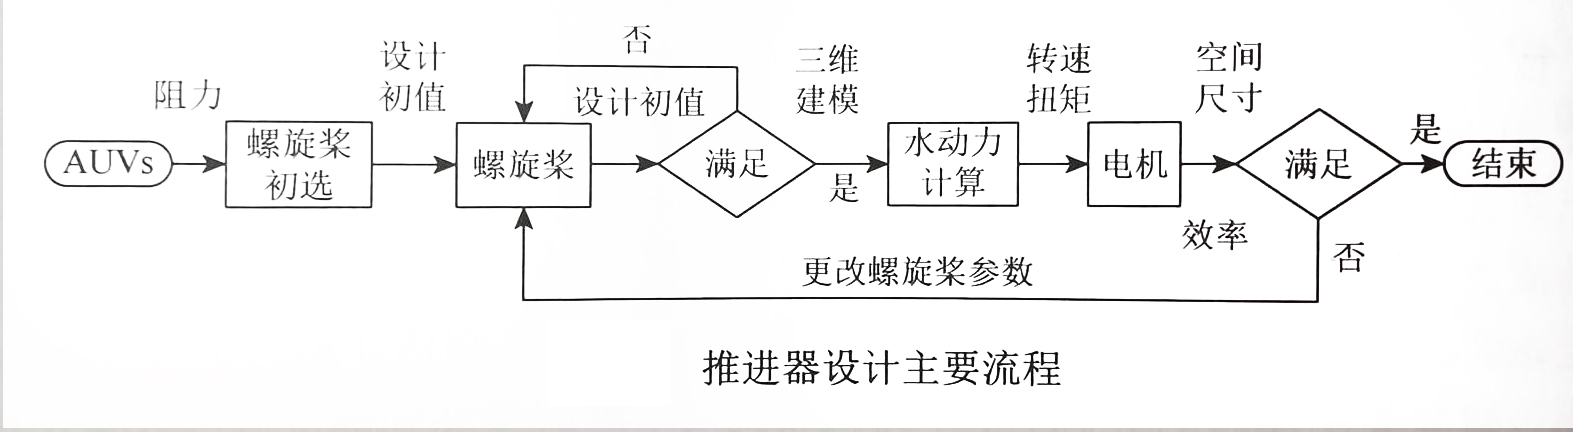
\includegraphics[scale=0.3]{./nengyuanyudongli.jpg}
推进系统在能量传输的过程中不可避免的有能量损耗,下面列出推进系统各效率成分与功率的关系:\\
\[\eta=\frac{P_E}{P_1}=\frac{P_E}{P_T}\frac{P_T}{P_{D0}}\frac{P_{D0}}{P_{DB}}\frac{P_{DB}}{P_S}\frac{P_S}{P_1}=\eta_H\eta_0\eta_R\eta_S\eta_J\]
因计算过于复杂及参数缺失,现结合资料估计效率为$\eta=0.8$.
\end{document}